\documentclass{article}
\usepackage[utf8]{inputenc}
\usepackage[spanish]{babel}
\usepackage{listings}
\usepackage{graphicx}
\graphicspath{ {images/} }
\usepackage{cite}

\usepackage[T1]{fontenc}

\usepackage{times}

\usepackage{color}
\definecolor{gray97}{gray}{.97}
\definecolor{gray75}{gray}{.75}
\definecolor{gray45}{gray}{.45}


\lstset{ frame=Ltb,
framerule=0pt,
aboveskip=0.5cm,
framextopmargin=3pt,
framexbottommargin=3pt,
framexleftmargin=0.4cm,
framesep=0pt,
rulesep=.4pt,
backgroundcolor=\color{gray97},
rulesepcolor=\color{black},
%
stringstyle=\ttfamily,
showstringspaces = false,
basicstyle=\small\ttfamily,
commentstyle=\color{gray45},
keywordstyle=\bfseries,
%
numbers=left,
numbersep=15pt,
numberstyle=\tiny,
numberfirstline = false,
breaklines=true,
}

% minimizar fragmentado de listados
\lstnewenvironment{listing}[1][]
{\lstset{#1}\pagebreak[0]}{\pagebreak[0]}

\lstdefinestyle{consola}
{basicstyle=\scriptsize\bf\ttfamily,
backgroundcolor=\color{gray75},
}

\lstdefinestyle{C++}
{language=C++}

\begin{document}

\begin{titlepage}
    \begin{center}
        \vspace*{1cm}
            
        \Huge
        \textbf{Desafío 1: Nada es lo que parece}
            
        \vspace{0.5cm}
        \LARGE
        Informa 2 S.A.S.
            
        \vspace{1.5cm}
            
        \textbf{Víctor Manuel Jiménez García\\
                José Miguel Jaramillo Sánchez\\
                Sebastián García Morales}

        \vfill
            
        \vspace{0.8cm}
            
        \Large
        Departamento de Ingeniería Electrónica y Telecomunicaciones\\
        Universidad de Antioquia\\
        Medellín\\
        Febrero 17 de 2022
    \end{center}
\end{titlepage}

\tableofcontents

\newpage
\section{Objetivos}\label{objetivos}
\begin{itemize}
    \item Aplicar los conocimientos adquiridos a lo largo del curso, demostrando apropiación de los fundamentos básicos del lenguaje de programación C++.
    \item Desarrollar habilidades de investigación y redacción que permitan la adquisición de nuevos conocimientos con el fin de solucionar problemas de la vida real.
    \item Demostrar la importancia y utilidad de la programación por hardware, así como el uso de módulos físicos para optimizar el uso de software en un diseño.
    \item Diseñar un aplicativo en la plataforma de Arduino integrando programación de C++ para solucionar un desafío  propuesto.
\end{itemize}
\section{Introducción}\label{intro}
\section{Marco Teórico}\label{marco}

\subsection{Conocimientos previos}

A la hora de enfrentarse a un desafío lo más recomendable es dividirlos en varias etapas para trabajarlo más fácilmente, una primera etapa sería realizar una investigación de conceptos y componentes propuestos en el desafío. En este caso es necesario investigar el concepto de transferir información de forma serial y paralela cómo también identificar características, funcionalidades, arquitectura, conexiones, alcances y limitaciones del circuito integrado 75HC595, por otro lado, ¿qué es un Arduino? Y ¿cómo unirlo al circuito integrado mencionado anteriormente para lograr solucionar el desafío completo?\\

Arduino es una plataforma de desarrollo basada en una placa electrónica de hardware libre que incorpora un microcontrolador reprogramable  y una serie de pines hembra. Estos permiten establecer conexiones entre el microcontrolador y los diferentes sensores y actuadores de una manera muy sencilla (principalmente con cables DuPont).\cite{arduinowebsite}\\

Este dispositivo es el que nos permitirá recibir los datos ingresados por el usuario y realizar la conversión a binario, además de funcionar tanto transmisor como receptor en el sistema de encoriación.\\

La comunicación entre Arduinos ser realizará de forma serial, que es el proceso de enviar datos de carácter binario un bit a la vez, esto provee la ventaja de mantener la interfaz transmisor - receptor de forma simple y eficiente.\cite{serialsite}\\
Por lo tanto, para desencriptar, es necesario paralelizar dicha secuencia de bits que luego serán las entradas de un circuito de lógica combinacional encargado de comparar los datos de acuerdo a los parámetros de desencriptación.

Paralelizar no es más que llevar la secuencia de bits que se desplazan como una sola fila, y transformarla en una columna. De esta forma si se tiene una secuencia serial de n bits, al paralelizar, el resultado es una columna de bits de n filas.

\begin{figure}[!ht]
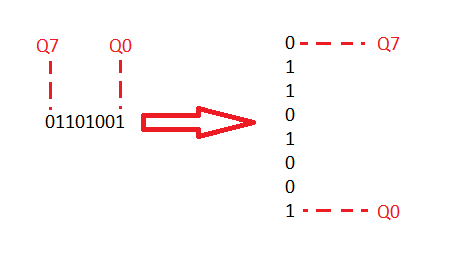
\includegraphics[width=8cm]{paralelizacion.png}
\centering
\caption{Ejemplo de paralelización}
\end{figure}

Esta acción de paralelizar la llevará a cabo el circuito integrado 74HC595 también conocido como Registro de desplazamiento. Este chip de 16 pines, recibe una secuencia de 8 bits en un solo pin, y los va almacenando en cada una de las salidas para luego ser liberados como 8 señales independientes.\\

Dos definiciones que se deben de tener en cuenta para entender mejor el funcionamiento de todo el sistema son: comunicación síncrona y comunicación asíncrona.\\

\noindent\textbf{Comunicación sincrónica:} Se da cuando el intercambio de mensajes sucede en tiempo real. Requiere que las dos partes (emisor y receptor) estén presentes en el mismo tiempo y espacio, ya sea físico o virtual. Por ejemplo, las llamadas telefónicas, las reuniones en la oficina o las videoconferencias.\\

\noindent\textbf{Comunicación asíncrona:} Sucede cuando los mensajes se intercambian sin importar el tiempo. Es decir, que no necesitan la atención inmediata del receptor, quien puede responder en el momento que decida o pueda hacerlo. Estamos hablando de medios como el correo electrónico, foros en línea, chats, mensajes de texto y documentos colaborativos.\cite{sincrosite}\\

En este caso, la comunicación se da de forma síncrona con ayuda de un pulso de reloj.
En electrónica y especialmente en circuitos digitales síncronos, una señal de reloj es una señal usada para coordinar las acciones de dos o más circuitos, esta señal oscila entre estado alto y bajo, también conocido como flanco de subida y de bajada, respectivamente, y gráficamente toma la forma de una onda cuadrada.\cite{relojsite}\\

\begin{figure}[!ht]
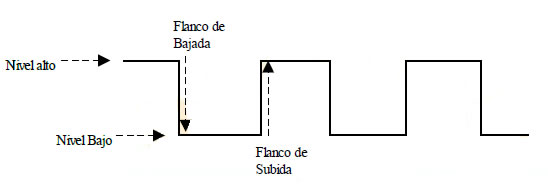
\includegraphics[width=8cm]{flanco1.jpg}
\centering
\caption{Diagrama de tiempo de una señal de reloj}
\end{figure}

A continuación se muestra la distribución de pines del circuito integrado 74HC595\\

\begin{figure}[!ht]
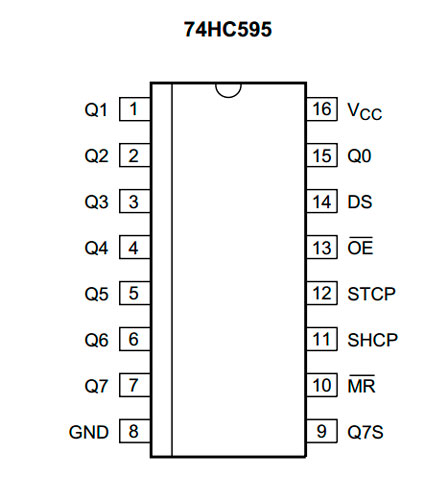
\includegraphics[width=5cm]{74HC595.jpg}
\centering
\caption{Pines IC 74HC595}
\end{figure}

\noindent\textbf{Entradas:}\\
\indent \textbf{GND} (pin 8): conexión a tierra (0 V)\\
\indent \textbf{GND} (pin 10): reinicio del registro (activo bajo)\\
\indent \textbf{SHCP} (pin 11): señal de reloj \\
\indent \textbf{STCP} (pin 12): pulso para liberar los datos \\
\indent \textbf{GND} (pin 13): habilitar salida del registro (activo bajo)\\
\indent \textbf{DS} (pin 14): entrada de datos serial \\
\indent \textbf{VCC} (pin 16): conexión a fuente de voltaje (5 V)\\

\noindent\textbf{Salidas:}\\ 
\indent \textbf{Q0-Q7} (pines 1-7 y 15 ): salida de datos\\
\indent \textbf{Q7S} (pin 9): salida de datos serial\\


El funcionamiento es el siguiente, la información serial entra por el \textbf{DS (pin 14)}, el integrado recibe cada bit cuando ocurre un flanco de subida por el \textbf{SHCP (pin 11)} y lo almacena en la salida de más bajo valor \textbf{Q0 (pin 15)}, a medida que van entrando más bits, los datos que se habían almacenado anteriormente se van desplazando desde \textbf{Q0} hasta \textbf{Q7} hasta completar el byte. Una vez hecho esto, se manda un flanco de subida en \textbf{STCP (pin 12)}, que se encarga de liberar los datos almacenados.\\

\noindent De esta forma el primer bit que entra, queda en la salida \textbf{Q7} y el último en la salida \textbf{Q0}.
Para ingresar un nuevo byte se debe borrar la información del registro, esto se hace mandando un flanco de bajada al pin \textbf{MR (pin 10)} y luego activando la salida del registro \textbf{(pin 12)}.\cite{74hc595datasheet}

\section{Análisis del problema} \label{analisis}

\subsection{Panorama del problema}


El problema consiste en transferir una secuencia de bits encriptados desde un Arduino a otro de forma serial, desencriptándola antes de que llegue al receptor usando lógica combinacional y un registro de desplazamiento.\\

Inicialmente, la información se dará al Arduino en forma de arreglo numérico ingresándola por la consola serial del microcontrolador, este se encargará de realizar la conversión a binario y de generar los pulsos de reloj y reset necesarios para usar en el circuito integrado 74HC595.\\

La salida serial del Arduino, así como las señales de sincronización entraran al 74HC595 que se encargará de paralelizar los datos, entregando 8 salidas diferentes, que a su vez alimentaran las compuertas de un circuito de lógica combinacional con una única salida True o False de acuerdo a una referencia dada.\\

Al Arduino receptor le entrarán el reloj y los datos en forma serial; sin embargo, solo admitirá aquella información que bajo ciertas condiciones dé como resultado un True en la lógica combinacional, en otras palabras, la lógica combinacional funcionará como un comparador que le dirá al receptor que información es correcta y cuál deberá ser descartada, realizando de esta forma la desencriptación de los datos.\\

\begin{figure}[!ht]
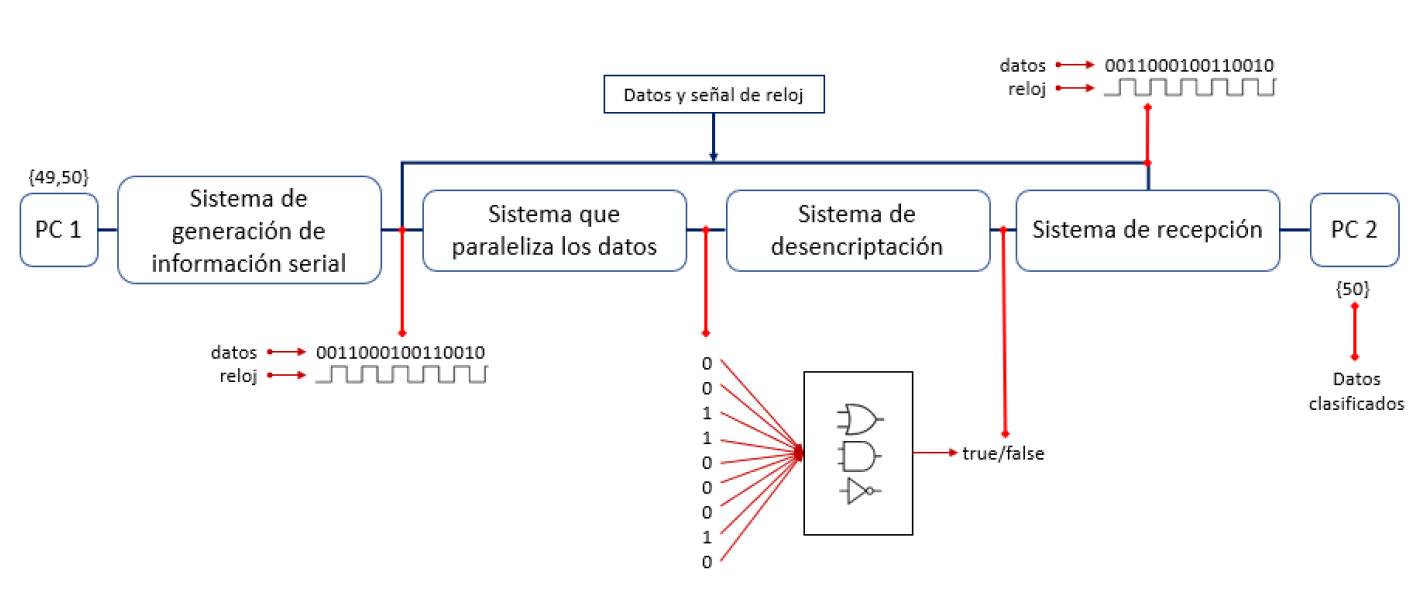
\includegraphics[width=10cm]{esquema.PNG}
\centering
\caption{Esquema del sistema a implementar. Recuperado de \cite{augusto}}
\end{figure}

En la siguiente sección se presentarán a detalle todas las etapas de solución.

\subsection{Etapas de la solución}

Para afrontar el problema, se opta por dividirlo en distintas etapas o módulos, de forma que se pueda verificar el correcto funcionamiento de cada uno por separado. Una vez hecho esto se juntan todas las etapas para posteriormente construir el modelo final del sistema.\\
\subsubsection{Circuito con el integrado 74HC595}

Como primera etapa se revisa el funcionamiento del circuito integrado 74HC595 en el simulador Tinkercad con ayuda de LEDS, botones y conmutadores. 

Para la alimentación se usa una fuente de voltaje de 5 V, se realizan las respectivas conexiones de forma que cada LED represente una salida del integrado y por facilidad se realiza el montaje solo para 4 bits. Las funciones de reloj, datos, y liberación de datos se realizan con conmutadores y botones.\\

Para ingresar un dato se usa el botón reloj, que permitirá la entrada de un 1 o un 0, de acuerdo a la posición que tenga los conmutadores deslizantes (la izquierda representa 1 y la derecha 0). Luego de tener 4 datos ingresados se presiona el botón reloj de registro, mostrando los datos ingresados en los leds.\\

Una vez montado el circuito, se evidencia que, aunque su comportamiento es el esperado, no se permitía ingresar más información nueva ni borrar la existente, esto se debía a que no se había agregado un botón de reset en el pin 10 del integrado. Esta corrección ya se muestra en el circuito de la Figura 5.\\

\begin{figure}[ht]
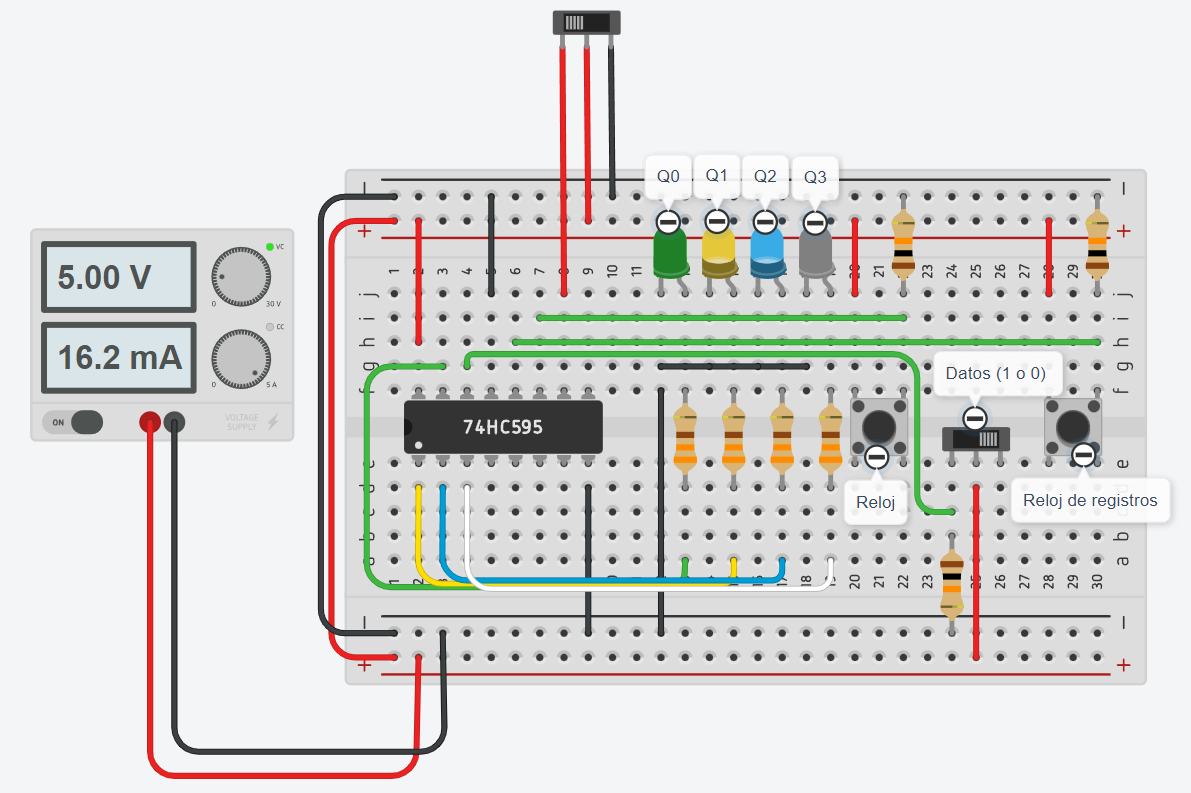
\includegraphics[width=7cm]{montaje0.PNG}
\centering
\caption{Primer montaje con el 74HC595}
\end{figure}

Después de haber garantizado el funcionamiento con botones y conmutadores, se procede a reemplazarlos por las salidas digitales del Arduino, en este caso el reset, el reloj de registro, la entrada de datos y el reloj están conectados a los pines 4, 5, 6 y 7 respectivamente. También se usan LEDS adicionales para llevar control de los pulsos que salen del Arduino como puede verse en la Figura 6.

El pulso de reloj principal es implementado internamente en el Arduino con ayuda de un ciclo y delays. Los datos a transmitir provienen de un arreglo de unos y ceros que es recorrido con un for y cuyo valor solo es liberado  cuando ocurre un flanco de subida del reloj. El reloj de registros tendrá un periodo de 4 veces el periodo del reloj principal, pues para este caso se está trabajando solo con 4 bits.


\begin{figure}[!ht] 
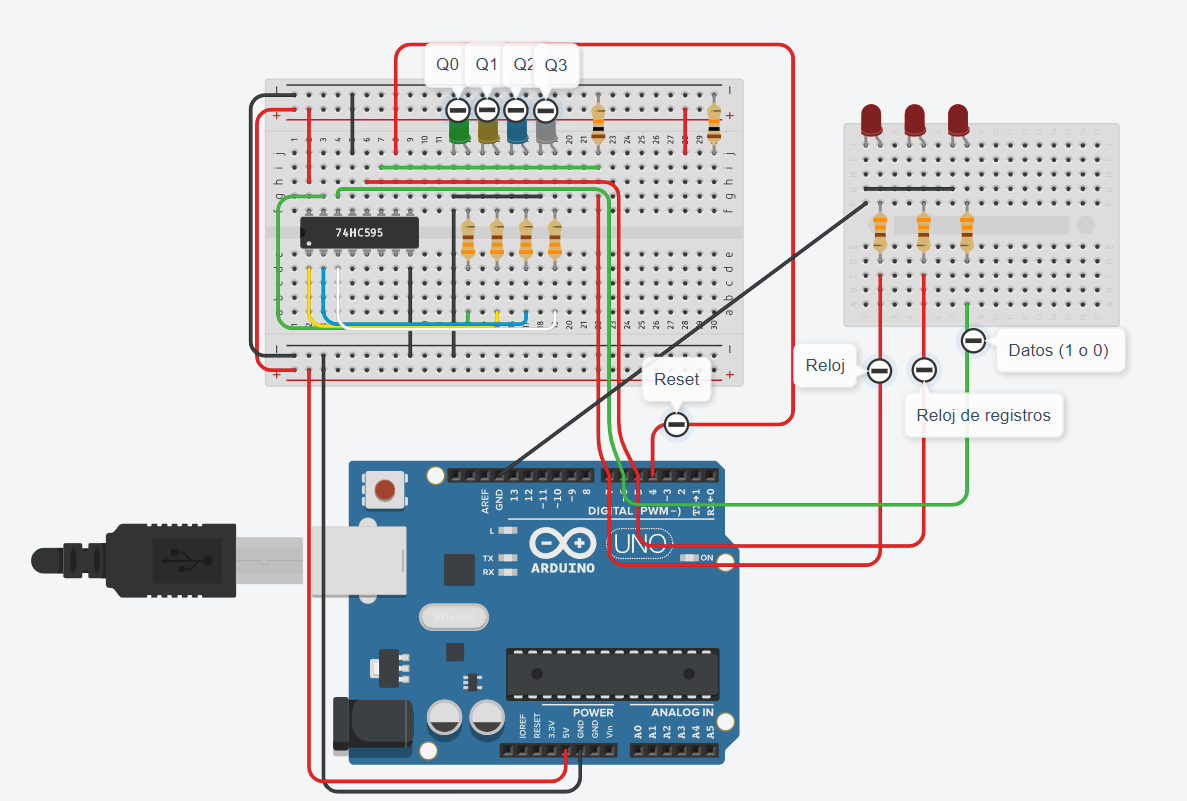
\includegraphics[width=7cm]{montaje1.PNG}
\centering
\caption{Montaje con 74HC595 y Arduino}
\end{figure}

\noindent
Código del Arduino con 74HC595:

\begin{lstlisting}[style=C++]
void setup()
{
  for(int i=4;i<8;i++){
  	pinMode(i, OUTPUT);
  }  
}
int binario[16]={0,0,0,1,0,1,1,0,0,1,1,0,1,0,0,0};
void loop()
{
  digitalWrite(4, LOW);
  digitalWrite(4, HIGH);
  digitalWrite(5, LOW);
  for(int i=0;i<16;i++){//debe recorrer todo el arreglo
    digitalWrite(5, LOW);
    if(binario[i]==1) digitalWrite(6, HIGH);
    else digitalWrite(6, LOW);
    delay(50);
    digitalWrite(7, HIGH);
    if((i+1)%4==0) digitalWrite(5, HIGH);//debe ser multiplo de la particion
    delay(450);
    digitalWrite(7, LOW);
    digitalWrite(5, LOW);
    digitalWrite(6, LOW);
    delay(500); 
  }
}
\end{lstlisting}

\subsubsection{Comunicación serial entre Arduinos}
Para enviar la información se usan dos pines digitales en cada Arduino, configurándolos como pines de entradas y salida para el receptor y transmisor respectivamente. Uno de los pines es para el reloj principal (pin 2 en el Arduino de la derecha)  y el otro para los datos en forma serial (pin 3 en el Arduino de la derecha). Los pulsos de reloj son generados internamente en el Arduino transmisor con ayuda de un ciclo y diferentes delay como se muestra en el código del Arduino 1 (TX-Izquierdo).
Se usa una variable global denominada tiempo que permite configurar el periodo de reloj y velocidad de transmisión de los datos.\\

En el Arduino receptor se usa un condicional que detecte si hay un flanco de subida en el reloj principal, y si lo hay se imprime en la consola serial 1 o 0 según el valor que haya en el pin de datos, ya sea un HIGH o un LOW. La impresión por consola es solo una medida de controlar el correcto funcionamiento del montaje, posteriormente los datos se usarán con otro objetivo como convertirlos a decimal.\\

Durante la implementación se presentó la dificultad de que el receptor tomaba varias veces el mismo valor debido a que la función loop se repite mucho más rápido de lo que cambian el reloj. Para solucionarlo, se redujo drásticamente el tiempo en alto del reloj hasta 0.5 ms, de forma que el receptor pueda recibir solo un dato a la vez y no varias veces el mismo dato generando errores. El montaje se muestra en la Figura 7.

\begin{figure}[!ht] 
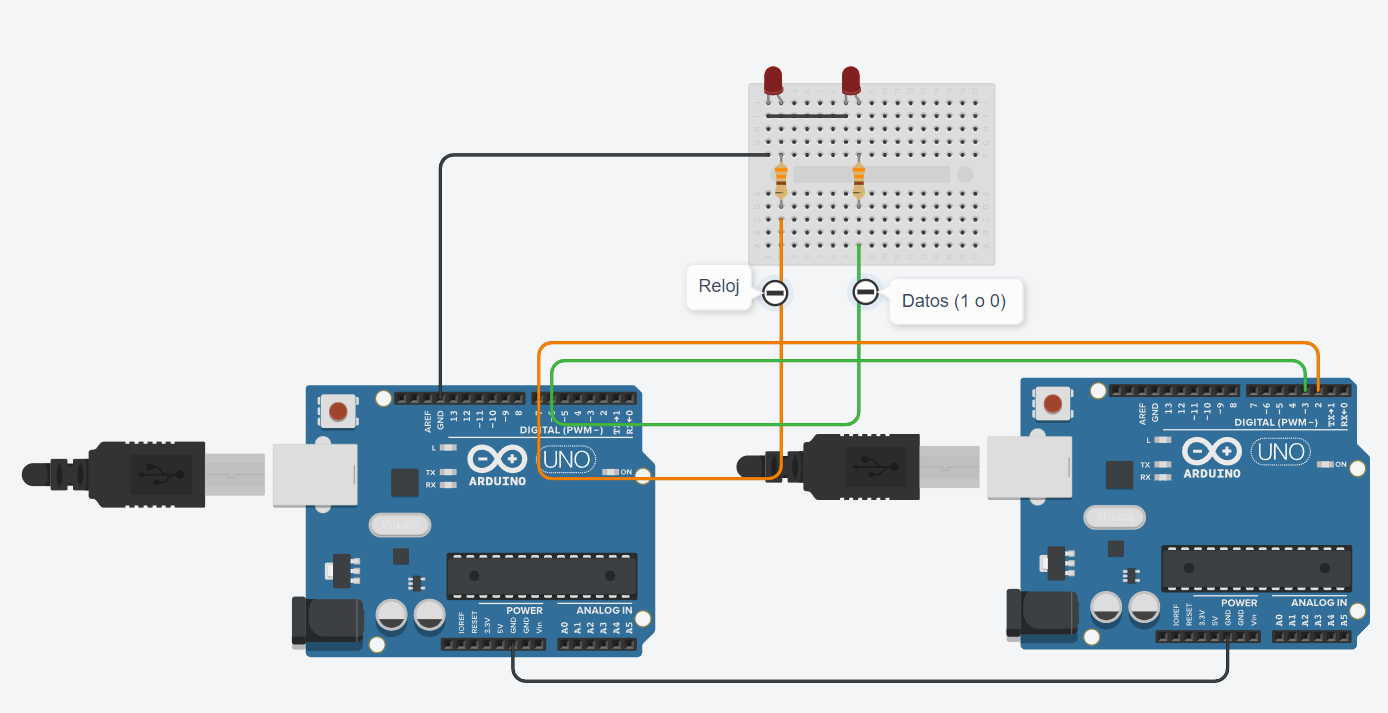
\includegraphics[width=7cm]{montajeSerial.PNG}
\centering
\caption{Montaje de Arduinos en comunicación serial}
\end{figure}

\noindent
Código del Arduino 1 (TX-Izquierdo):

\begin{lstlisting}[style=C++]
void setup()
{
  for(int i=4;i<8;i++){
  	pinMode(i, OUTPUT);
  }  
}
int binario[24]={0,1,0,1,1,1,1,1,0,1,0,0,0,1,0,1,0,1,1,1,1,1,1,1};
int tiempo=500;//variable tiempo que define el periodo del reloj
void loop()
{
  digitalWrite(4, LOW);
  digitalWrite(5, LOW);
  digitalWrite(4, HIGH);
  for(int i=0;i<24;i++){//debe recorrer todo el arreglo
    digitalWrite(5, LOW);
    if(binario[i]==1) digitalWrite(6, HIGH);
    else digitalWrite(6, LOW);
    delay(tiempo/20);//50
    digitalWrite(7, HIGH);
    if((i+1)%8==0) digitalWrite(5, HIGH);//debe ser multiplo de la particion
    delay(0.5); //un tiempo muy bajo de reloj, garantiza que solo se tome un dato en el otro Arduino
    digitalWrite(7, LOW);
    delay(tiempo-tiempo/2-tiempo/20-0.5);
    digitalWrite(5, LOW);
    digitalWrite(6, LOW);
    delay(tiempo/2); 
  }
}
\end{lstlisting}

\noindent
Código del Arduino 2 (RX-Derecho):

\begin{lstlisting}[style=C++]
void setup()
{
  for(int i=2;i<4;i++){
  	pinMode(i, INPUT);
  } 
  Serial.begin(9600);
}
bool dato=LOW,datoAnterior=LOW;
void loop()
{
  dato=digitalRead(2);
  if(dato==HIGH && datoAnterior==LOW){ //detector de flancos
  	if(digitalRead(3)==HIGH) Serial.println(1);
    else if(digitalRead(3)==LOW) Serial.println(0);
  }
  datoAnterior==dato;
  Serial.println(1);
}
\end{lstlisting}

\subsubsection{Módulo de desencriptación}
El módulo de desencriptación consiste en un circuito de lógica combinacional que compara los 8 bits que salen del 74HC595 con los 8 bits del número de referencia que en nuestro caso es el \textbf{127}.\\

Para comparar bit a bit se requieren 8 compuertas XOR, en una de las entradas entra el bit que sale del integrado, y en la otra entrada el bit correspondiente al número de referencia. Según la tabla de verdad de la compuerta XOR, mostrada en la Figura 8, cuando ambas entradas son iguales, la salida es cero, por tanto, se usan negadoras para que cuando esto ocurra se tenga un valor True en la salida, de esta forma se requieren 8 compuertas NOT. Las 8 salidas de las negadoras alimentan la entrada de un sistema de compuertas AND cuyo objetivo es comparar que todas las salidas de las NOT sean 1, es decir, que todos los bits sean iguales, por lo que se necesitan 7 compuertas AND.\\


\begin{figure}[!ht] 
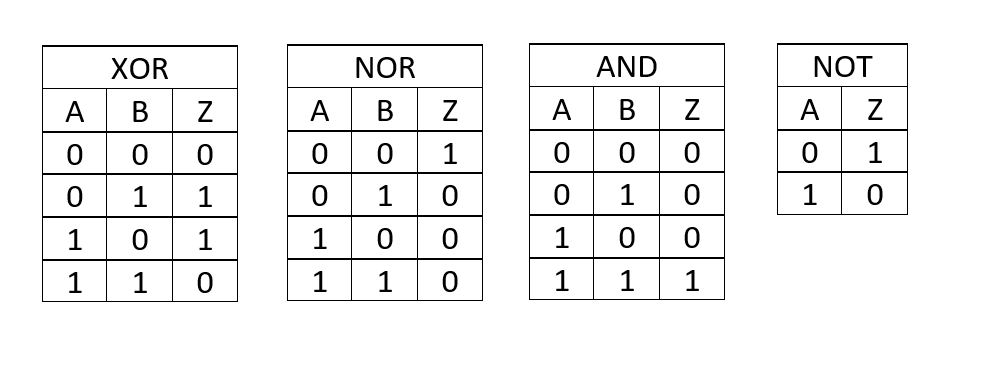
\includegraphics[width=10cm]{compuertas.png}
\centering
\caption{Tablas de verdad de las compuertas XOR, NOR, AND y NOT}
\end{figure}

Dentro del catálogo de integrados de compuertas lógicas disponibles en el aplicativo Tinkercad tenemos los siguientes:
\begin{itemize}
    \item 74HC21: dos compuertas AND de 4 entradas
    \item 74HC08: 4 compuertas AND de dos entradas
    \item 74HC86: 4 compuertas XOR de dos entradas
    \item 74HC02: 4 compuertas NOR de dos entradas
    \item 74HC04: 6 compuertas negadoras\\
\end{itemize}

De esta forma, y considerando integrados que solo dispongan de compuertas de dos entradas se necesitarían alrededor de 6 integrados en total para realizar el montaje planteado en la Figura 9.

\begin{figure}[!h] 
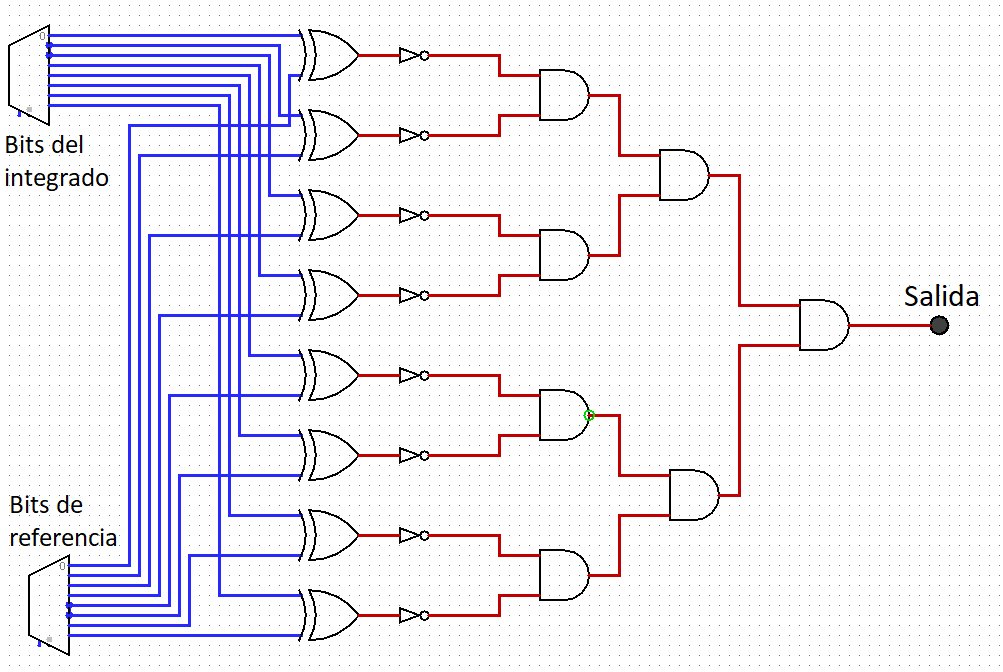
\includegraphics[width=8cm]{logica1.png}
\centering
\caption{Circuito de lógica combinacional propuesto}
\end{figure}

Analizando un poco mejor el circuito y usando álgebra de bool, se observa que la expresión correspondiente a las AND cuyas entradas son negadas, puede transformarse aplicando la ley de De Morgan así: $\bar{A}\bar{B} = \overline{A+B}$.

Con esto estamos sustituyendo la AND y las negadoras, por una sola compuerta NOR y reduciendo el número de integrados de 6 a 4. También se puede usar una compuerta AND de 4 entradas para reemplazar las 3 AND de 2 entradas en la parte final del circuito. Aunque esto no reduce los integrados a usar, sí facilita la conexión de los chips durante el montaje. Esta simplificación se muestra en la Figura 10.

\begin{figure}[!hb] 
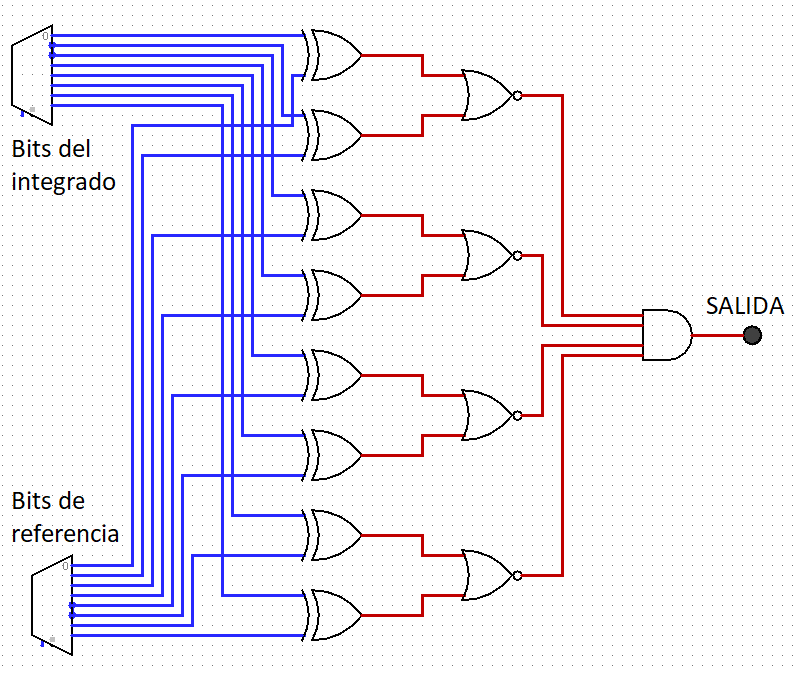
\includegraphics[width=8cm]{logica2.png}
\centering
\caption{Circuito de lógica combinacional simplificado}
\end{figure}

Con el esquema planteado, se monta el circuito en Tinkercad, usando una fuente de alimentación de 5 V, DIP conmutadores para simular las entradas, los integrados de compuertas lógicas \textbf{74HC86 (XOR)}, \textbf{74HC02 (NOR)}, \textbf{74HC21 (AND)} y un diodo LED que se enciende cuando ambos números son iguales.\\

\begin{figure}[!ht] 
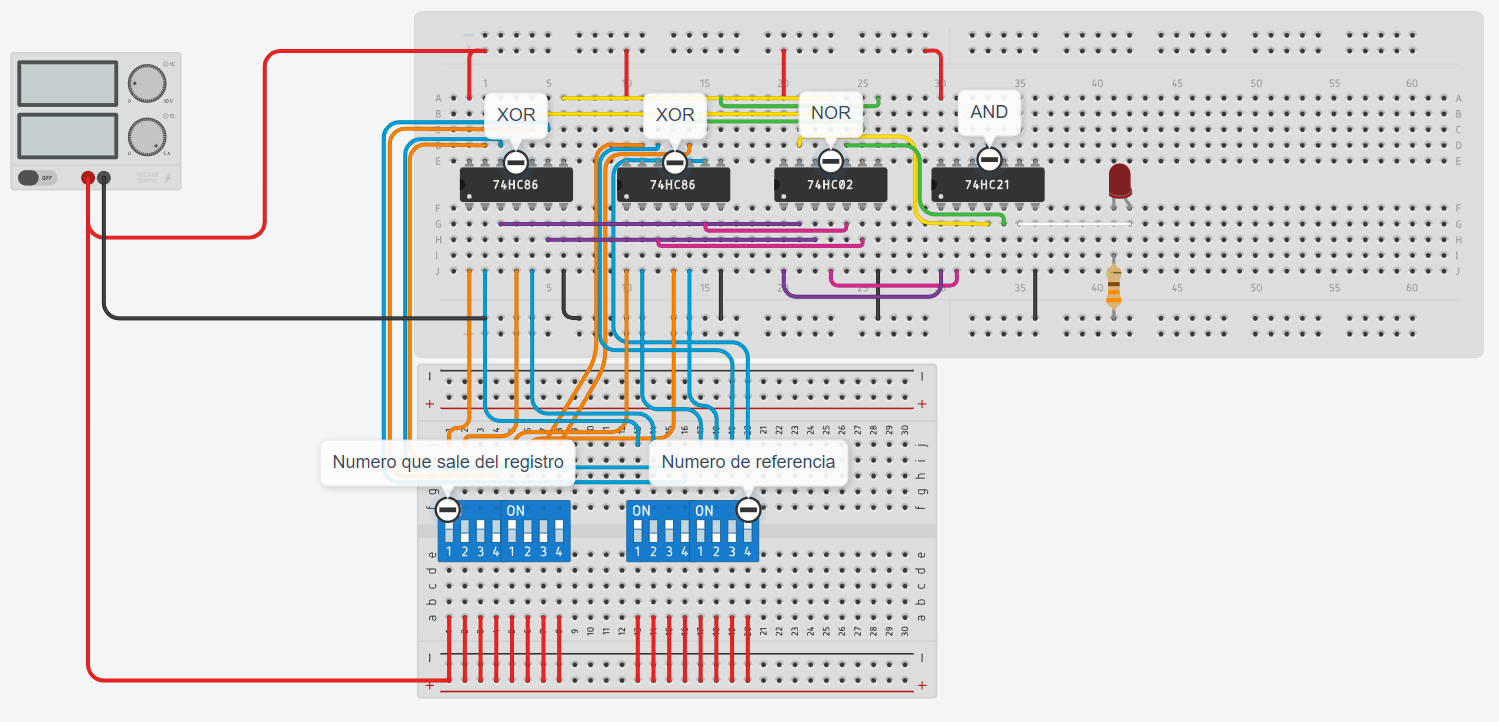
\includegraphics[width=10cm]{montajeCompuertas.PNG}
\centering
\caption{Implementación del circuito de lógica combinacional simplificado}
\end{figure}

Para la construcción final, el DIP conmutador "Número que sale del registro" será reemplazado por las 8 salidas del 74HC595 (Registro de desplazamiento), mientras que el otro DIP conmutador no cambiará, y siempre tendrá el número de referencia 127, o cualquier otro pedido durante su ejecución.
\subsubsection{Conversión de entero a binario en Arduino}
Debido a que en el problema, se entrega un arreglo de enteros es necesario elaborar un programa que realice la conversión de decimal a binario. Inicialmente, la implementación se realiza en QT, para apoyarse del depurador y realizar pruebas. Posteriormente, se lleva el código al Arduino transmisor. El código se encuentra a continuación:

\noindent


\begin{lstlisting}[style=C++]
#include <iostream>
using namespace std;

//Programa que convierte un arreglo de enteros a un arreglo binario
int main()
{
    int tam=11, n, num[11]={49,67,13,240,50,89,17,93,170,127,28};
    int *bin = new int[8*tam];
    for (int i=0,test=1;i<tam;i++, test++) {
        n=num[i];
        for (int j=7,k=8*test-1;j>-1;j--) {
            if (n%2==0) {
                bin[k]=0; //se empieza a llenar desde la posicion final de la particion de 8 bits
            }
            else{
                bin[k]=1;
            }
            n/=2;
            k--;
        }
    }
    for (int i=0;i<tam*8;i++) {//Imprime el arreglo (CONTROL)
        cout<<*(bin+i);
        if((i+1)%8==0) cout<<"|";//Separador de bits
    }
    cout<<endl;
    delete[] bin;
    return 0;
}
\end{lstlisting}

El código consiste en un for que recorre el arreglo de enteros, y a cada elemento le realiza la división sucesiva por dos para obtener la conversión a binario. El arreglo de bits se llena de forma tal que el bit más significativo quede a la derecha de cada partición de 8 bits.
En la parte final se tiene un ciclo que imprime el arreglo para comprobar que todo está correcto.

\subsubsection{Ensamble de los modulos anteriores}
Una vez garantizado el correcto funcionamiento de cada módulo por separado, se procede a ensamblarlos y realizar las conexiones respectivas. Primero se reemplazó el DIP conmutador que simulaba la salida de los datos del integrado en el módulo de encriptación, por las salidas reales del 74HC595. Luego se conectaron ambos Arduinos y se cargaron los códigos para permitir la comunicación serial. Se optó por conservar algunos montajes de LED como elementos de control. El montaje se puede apreciar en la Figura 12.

\begin{figure}[!ht] 
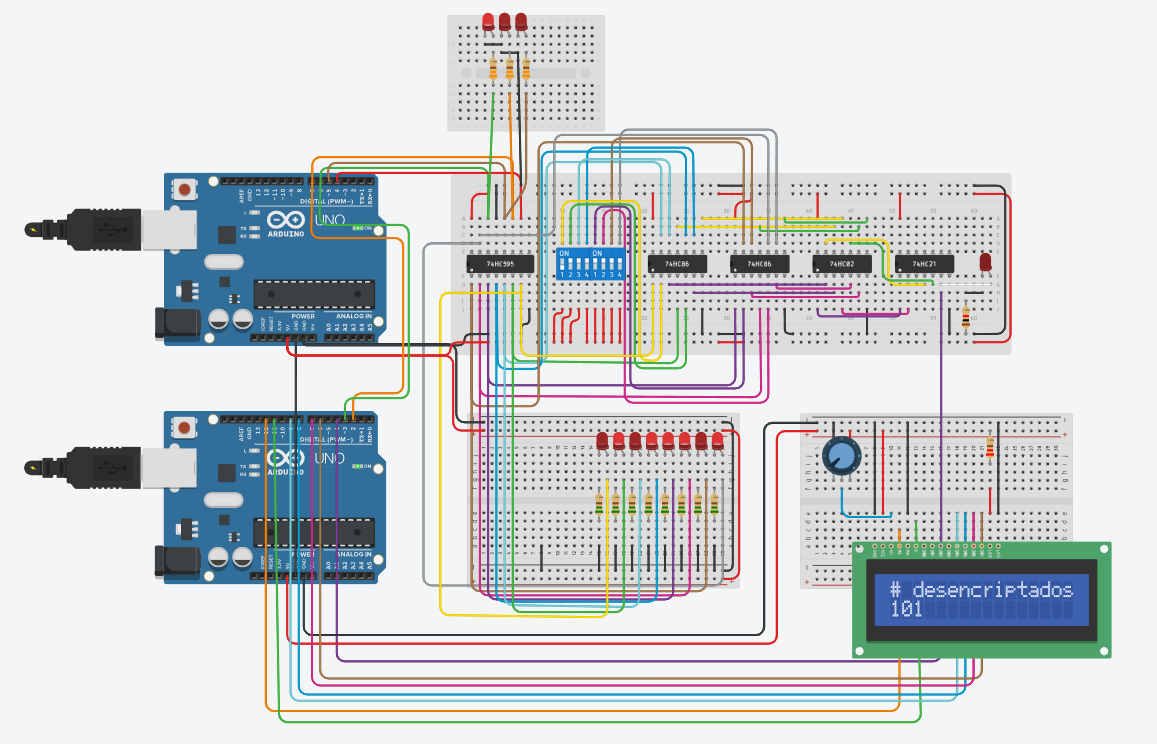
\includegraphics[width=12cm]{esquemaEnsamble.PNG}
\centering
\caption{Ensamble de los módulos anteriores}
\end{figure}



\section{Conclusiones} \label{conclusiones}

\bibliographystyle{IEEEtran}
\bibliography{references}

\end{document}
